\section{Blockchain}
\label{sec:blockchain}

La blockchain come dice il nome è una catena di blocchi che implementano un database  aperto e distribuito, atto a memorizzare le transazioni tra due parti in modo sicuro, verificabile e permanente. In altre parole, la blockchain rappresenta il libro contabile (o libro mastro), ossia il registro sul quale sono riportati tutti gli scambi tra le parti. Questo libro mastro è distribuito (Distributed Ledger) replicato e sincronizzato tra tutti i membri di una rete. In questo database vengono registrate le transazioni (come lo scambio di beni o informazioni) tra i partecipanti alla rete.
\\I dati non sono memorizzati su un solo computer ma su più macchine collegate tra loro attraverso una rete peer-to-peer [\ref{fig:blockchainNetwork}] sottoforma di blocchi.
\\Ciascun nodo è autorizzato ad aggiornare e gestire il libro contabile distribuito in modo indipendente, ma sotto il controllo consensuale degli altri nodi. Infatti, gli aggiornamenti non sono più gestiti, come accadeva tradizionalmente, sotto il controllo rigoroso di un’autorità centrale, ma sono invece creati e caricati da ciascun nodo in modo appunto indipendente. In questo modo ogni partecipante è in grado di processare e controllare ogni transazione ma, nello stesso tempo ogni singola transazione, essendo gestita in autonomia, deve essere verificata, crittografata e approvata dalla maggioranza dei partecipanti alla rete. 

\begin{figure}[H]
	\centering
	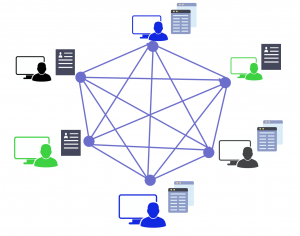
\includegraphics[width=0.5\textwidth]{images/blockchainNetwork.png}
	\caption{Rete distribuita di nodi paritari.}
	\label{fig:blockchainNetwork}
\end{figure}

Ogni blocco contenuto nella blochchain archivia un insieme di transazioni validate correlate da un Marcatore Temporale (Timestamp) ed un hash (una stringa alfanumerica) che identifica il blocco in modo univoco e che permette il collegamento con il blocco precedente[\ref{fig:blockChain}].

\begin{figure}[H]
	\centering
	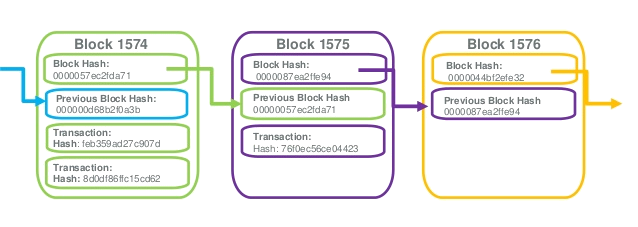
\includegraphics[width=\textwidth]{images/blockChain.png}
	\caption{Catena di blocchi nella blockchain.}
	\label{fig:blockChain}
\end{figure}

Perché un nuovo blocco di transazioni sia aggiunto alla Blockchain è necessario appunto che sia controllato, validato e crittografato. Solo con questo passaggio può poi diventare attivo ed essere aggiunto alla Blockchain. Per effettuare questo passaggio è necessario che ogni volta che viene composto un blocco venga risolto un complesso problema matematico che richiede un cospicuo impegno anche in termini di potenza e di capacità elaborativa. Questa operazione viene definita come “Mining” ed è svolta dai “Miner”. La risoluzione del problema è un processo irreversibile per cui il blocco valido aggiunto alla catena diviene immutabile.
\\In conclusione, questa tecnologia può essere utilizzata in tutti gli ambiti in cui è necessaria una relazione tra più persone o gruppi. Ad esempio può garantire il corretto scambio di titoli e azioni o sostituire un atto notarile, perché ogni transazione viene sorvegliata da una rete di nodi che ne garantiscono la correttezza senza l’ausilio di intermediari.
\\Bitcoin sfrutta questa tecnologia per gestire le transazioni finanziarie in modo sicuro e del tutto autonomo.